% Note that the text in the [] brackets is the one that will
% appear in the table of contents, whilst the text in the {}
% brackets will appear in the main thesis.

%% CHAPTER HEADER /////////////////////////////////////////////////////////////////////////////////////
\chapter[Concept of the Method]{Concept of the Method}
\label{ch:method}

%% CHAPTER INTRODUCTION ///////////////////////////////////////////////////////////////////////////////
The Chapter presents the research methodology used in the dissertation to determine the validity of the thesis. 
First, a discussion of different methods for numerical modelling \ac{gw} propagation in \ac{hsc} is provided. 
Then a framework of the new model is presented, complemented by the description of methods for determining the material properties of each component for varied ambient temperatures.
The Chapter also describes the proposed model-assisted damage severity assessment approach.
%% INCLUDE SECTIONS ///////////////////////////////////////////////////////////////////////////////////
%% SECTION HEADER /////////////////////////////////////////////////////////////////////////////////////
\section{Modeling of the \acs{gw} propagation in the \acsp{hsc}}
\label{sec:modelling}

%% SECTION CONTENT ////////////////////////////////////////////////////////////////////////////////////

%% SUBSECTION HEADER //////////////////////////////////////////////////////////////////////////////////

In the dissertation, the \ac{hsc} composed of an aluminium honeycomb core and the skin made of \ac{cfrp} is assumed for further analysis.
The most common numerical modeling of the phenomenon of \ac{gw} in the \acp{hsc} found in the literature is a calculation of the effective material properties of the honeycomb structure \cite{baid2015dispersion, mustapha2014leaky, qi2008ultrasonic,  shi1995derivation, sikdar2016guided}.
The properties are obtained from the analytical \cite{gibson1982mechanics, malek2015effective} or the \ac{fem} \cite{catapano2014multi, chen2014analysis} analysis of the honeycomb \ac{rve}.
A comprehensive literature review on the homogenisation of the honeycomb structure is presented in the work of Ahmed \cite{ahmed2019homogenization}.
Replacing the core geometry with a homogeneous material has many advantages.
First and foremost, it simplifies the domain mesh so that convergence of the solution requires fewer working memory resources and increases the value of the critical time step.
In addition, the wave propagation velocity determined by the simulation is in good agreement with the experiment.

However, this method cannot adequately represent the phenomenon of propagating wave interaction in honeycomb cells.
It causes the signal energy not to dissipate as it would in a real structure.
A more precise model is the \ac{fcgm}. 
Ruzzene et al. presented a parametric study to evaluate the dynamic behavior of the honeycomb and cellular structures through the \ac{fem} and the application of the theory of periodic structures \cite{ruzzene2003wave}.
Recently, the simulations of the wave propagation in the \acp{hsc} have been conducted with commercially available finite element codes~\cite{song2009guided, hosseini2013numerical, tian2015wavenumber, zhao2018wave}.

While the \ac{fem} based modelling of \ac{gw} requires a significant amount of memory and is time-consuming, this method becomes inefficient in the case of \ac{fcgm}.
Kudela increased the computational efficiency with the model based on the time-domain \ac{sem} \cite{kudela2016parallel}.
In addition, the algorithm has been adapted for parallel computing on the \ac{gpu}, making the simulations 14 times faster than on the \ac{cpu}.
However, this approach has two major drawbacks. One is employing solid elements with three \acp{dof} at each node to model the core walls. As a result, a \numproduct{179 x 160} \unit{\square\mm} sandwich panel has over 1.5 million \acp{dof}.
Secondly, no \ac{pzt} sensors were considered in the simulation, so a concentrated force was used to generate the \ac{gw}.
To attach the transducers, the grids of the sensor and the host plate must coincide or use an interface between them. 

The disadvantages of existing modelling methods, motivated me to propose a new model of the \ac{hsc}.
In the proposed model, the core of the plate consists of \ac{2d} elements, one per cell wall.
Since the neutral plane of the elements is oriented differently concerning the global coordinate system, the local displacements vector has to be transformed accordingly.
The skin model is developed according to the laminate theory presented by Vinson and Sierakowski \cite{vinson1993behavior}.
In addition, two interfaces are used to connect the individual \ac{hsc} components.
One with the non-matching grid was developed to join the sensors with the panel.
It was done with the novel method based on the element shape functions described in Chapter \ref{ch:sem}.
The core and skin connection was implemented with a perfect matching interface.
To the best of my knowledge, the presented model has not been implemented yet for the \acp{hsc}.

The parametric study conducted in the dissertation leads to the determination of a \ac{madif}, which defines the influence of the composite defect size on wave propagation.
In this case, the defect is assumed to be a disbond between the skin and the core.
%% SECTION HEADER /////////////////////////////////////////////////////////////////////////////////////
\section{Temperature Effect on the GW Propagation}
\label{sec:temp}

%% SECTION CONTENT ////////////////////////////////////////////////////////////////////////////////////

%% SUBSECTION HEADER //////////////////////////////////////////////////////////////////////////////////
In order to carry out the temperature dependent SE simulation and semi-analytical analysis of Lamb wave propagation in the \acp{hsc}, the elastic modulus of \acp{hsc} layers are calculated as per the methodology described in \cite{chamis1983simplified,salamone2009guided}. The calculation is done for a range of temperature (+50\(^{\circ}\)C to -50\(^{\circ}\)) generally occurred in practical operating scenarios. The obtained temperature-dependent elastic properties (E11 = E22, E33, G12, G13 = G23) for composite laminate and adhesive (E, G) are presented in Figure 7 and Figure 8, respectively.

In this model \cite{salamone2009guided}, reduction of Young’s modulus of resin \(E_m\) with variation in temperature is assumed as:
\begin{eqnarray}
	E_m(T)=F_m E_{rm},
	\label{eq:factor_temp}
\end{eqnarray}
where \(E_{rm}\) is the Young’s Modulus of resin at the reference temperature and \(F_m\) is the temperature degradation factor as proposed in \cite{chamis1983simplified}:
\begin{eqnarray}
F_m=\sqrt{\frac{T_{g0}-T}{T_{g0}-T_r}},
\label{eq:em_temp}
\end{eqnarray}
where \(T_{g0}\) is the glass transition temperature and \(T_r\) is the reference temperature. In the study, the value of \(T_{g0}=215^{\circ}C\) and \(T_r=20^{\circ}C\) is selected from Table 2 in \cite{chamis1983simplified}. 

%% SECTION HEADER /////////////////////////////////////////////////////////////////////////////////////
\section{Model-assisted damage severity assessment}
\label{sec:madif}

%% SECTION CONTENT ////////////////////////////////////////////////////////////////////////////////////

%% SUBSECTION HEADER //////////////////////////////////////////////////////////////////////////////////
The process of determining the damage size is shown in the flowchart in Figure \ref{fig:Flowchart} \cite{fiborek2021model}.
Before inspecting a given \ac{hsc} panel, a numerical analysis has to be performed to determine a function that describes the effect of damage on wave propagation.
Then the model is subjected to experimental validation.
If the simulation results did not agree with the measured results, the material parameters of the components were adjusted.
In the dissertation, the \ac{cfrp} volume fraction of reinforcing fibres was adjusted to determine a wave velocity \cite{kudela2007modelling} and a damping coefficient of the skin to set the magnitude of the registered signals \cite{wandowski2017guided}.
\begin{figure}[!tbh]
	\begin{center}
		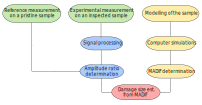
\includegraphics[width=0.95\textwidth]{Chapter_3/flowchart}
	\end{center}
	\caption{A flowchart representing the process for damage size estimation}
	\label{fig:Flowchart}
\end{figure}
\clearpage
When the structure model was developed, several computer simulations for various damage sizes were conducted to determine the \ac{madif}, a cornerstone of the dissertation. This function determines the severity of \ac{hsc} damage based on the signal received by the sensor.
Several excitation signals and damage indices were considered to select the best \ac{madif}.
The selection criterion was the monotonicity and the function slope over the considered range of the damage size. Then, the damage magnitude was obtained from the \ac{madif} for the measured signal and normalised to the reference one.
%%% SECTION HEADER /////////////////////////////////////////////////////////////////////////////////////
\section{Conclusions}
\label{sec:conclusionsMethod}

%% SECTION CONTENT ////////////////////////////////////////////////////////////////////////////////////



